\documentclass[11pt]{article}
% packages
\usepackage[french]{babel}

\usepackage[utf8]{inputenc}
\usepackage{geometry}
\usepackage[pdftex]{graphicx}
\usepackage{tabularx}
\usepackage{dsfont}
\usepackage{multirow}
\usepackage{amsmath,amsfonts,amssymb}
\usepackage{subcaption}
\usepackage{authblk}
%hyperlinks options
\usepackage{hyperref}
\hypersetup{colorlinks=true,linkcolor=blue,filecolor=magenta,urlcolor=cyan,citecolor=cyan}
%bib options
\usepackage[backend=biber,style=authoryear,bibstyle=authoryear,natbib=true,
giveninits=true,uniquename=false,uniquelist=false,% firstinits=false,
maxcitenames=2,date=year, maxbibnames=99,url=false]{biblatex}
\geometry{left=20mm, top=20mm, right=20mm}
%float barrier
\usepackage{placeins}
\addbibresource{Thèse.bib}
\title{Introduction}
\author{Mathieu}


\begin{document}
\maketitle

\tableofcontents

\newpage

\section{Contexte général}

	\paragraph{} L'inondation est le type de catastrophe naturelle le plus fréquent dans le monde, mais également celui ayant affecté le plus de personnes au cours des 20 dernières années \citep{undrr_human_2020}. Depuis le début du XXI\textsuperscript{ème} siècle, plus de 100 000 personnes ont perdu la vie dans des inondations à travers le globe. En France, il s'agit du premier risque naturel par l'importance des dommages provoqués et le nombre de communes concernées \citep{medd_prevention_2023}. Les inondations peuvent avoir des origines variées : crues, submersions marines, ruissellement, rupture de poche glaciaire, rupture d'ouvrage, etc. Parmi ces différents phénomènes, la crue est le type d'inondation le plus fréquent. 
	
	\paragraph{} Les hydrologues utilisent les chroniques de débit enregistrées en continu aux stations limnimétriques afin de caractériser statistiquement le risque de crue. Cette approche probabiliste, nommée prédétermination, consiste à anticiper la magnitude d'un événement futur ainsi que sa probabilité d'occurrence, mais sans en définir une date d'occurrence, ce qui diffère du concept de prévision. La notion de probabilité d'occurrence est intimement liée au concept de "période de retour", qui est également utilisé dans de nombreux domaines liés aux risques naturels. La période de retour découle de la notion statistique de probabilité au non-dépassement : on peut dire que le débit d'une crue de période de retour $T$ (en années) est en moyenne égalé ou dépassé toutes les $T$ années. On peut également dire qu'un débit de période de retour $T$ a une probabilité $p_1 = 1/T$ d'être dépassé chaque année, ou bien une probabilité $p_2 = 1-1/T$ de ne pas être dépassé. Il faut noter que ces affirmations ne sont valables qu'à condition que les processus à l'origine des crues soient stationnaires dans le temps. Même si il parait trivial, le concept de période de retour porte souvent a confusion. Par exemple, si la dernière crue centennale de la Seine ($T = 100$ ans) a eu lieu en 1910, cela n'a aucune conséquence sur la probabilité d'observer une crue centennale de la Seine en 2010. Cette probabilité reste en effet égale à $p = 1/100$, que l'on soit en 1910, 2010 ou 2023. A l'inverse, il est tout à fait possible d'observer deux crues centennales deux années de suite. La notion de période de retour est utilisée pour dimensionner des infrastructures ou pour protéger les populations en fonction du risque de crue dans la zone, en tenant compte d'une marge. Par exemple, en France, l'aléa de référence pris en compte dans le Plan de Prévention du Risque Inondation (PPRI) "correspond à un phénomène ayant une probabilité de survenance de 1 chance sur 100 chaque année. S'il existe une crue historique dont la période de retour est supérieure à la crue centennale, cet événement historique est retenu comme aléa de référence". \citep{medd_site_nodate}. Étant donné qu'il y a environ 63\% de chances d'observer au moins une crue centennale en 100 ans, on peut considérer que des infrastructures protégeant les populations jusqu'à la crue centennale auront environ 37\% de chances de couvrir efficacement leur rôle de protection au cours d'une période de 100 ans. La détermination précise du débit correspondant à une période de retour donnée (également appelé "crue de projet" ou "quantile de crue") est donc essentielle.
	
	\paragraph{} A l'origine, l'estimation des quantiles de crues était purement empirique. Il s'agissait par exemple, pour une station de mesure donnée, de calculer la fréquence cumulée des débits maximum annuels, classés par ordre croissant. On pouvait alors accéder à de premières estimations de la probabilité au non-dépassement pour un débit donné. Cependant, cette approche comporte de nombreuses limitations, notamment quand il s'agit d'extrapoler au delà du plus fort débit connu. Désormais, la pratique courante, appelée analyse fréquentielle des crues, consiste à estimer les paramètres d'une distribution statistique (préalablement choisie selon la variable hydrologique étudiée) en se basant sur les observations. Cette pratique comporte l'avantage, par rapport aux estimations empiriques, d'être moins sensible à la taille de l'échantillon d'observations disponible. De plus, elle offre la possibilité d'extrapoler au delà de la plus forte crue connue, ce qui permet d'accéder à de grandes périodes de retour qui sont nécessaires pour le dimensionnement d'infrastructures (par exemple jusqu'à $T =$ 10 000 ans pour les barrages français \citep{le_delliou_recommandations_2014}). 

	\paragraph{} Une autre grande famille de méthodes d'analyse fréquentielle se base sur les précipitations pour définir la distribution des crues. L'hypothèse derrière ces méthodes est que, sous certaines conditions de saturation du bassin versant, la distribution des débits extrêmes est bornée et dépend uniquement de la distribution des pluies extrêmes. On peut notamment citer à ce sujet les méthodes françaises GRADEX \citep{guillot_methode_1967} ou AGREGEE \citep{margoum_estimation_1994}. D'autres méthodes plus approfondies utilisent les mêmes hypothèses et se basent sur le couplage un générateur stochastique d'événements de pluies extrêmes avec un modèle hydrologique afin d'obtenir une meilleure description de la réponse des bassins versants. On peut notamment citer à ce propos la méthode française SCHADEX développée par EDF (Électricité De France) \citep{paquet_schadex_2013}. Des méthodes d'analyse fréquentielle classiques seront utilisées tout au long de ce manuscrit, mais l'utilisation de méthodes pluie/débit auraient également pu répondre à certaines problématiques de la thèse. Cependant, elles ne sont pas réellement adaptées à l'analyse historique des crues. Il faut noter qu'il n'existe pas de consensus scientifique en faveur des méthodes classiques d'analyse fréquentielle (basées uniquement les chroniques de débit), ou en faveur des méthodes pluie/débit.
				
	\paragraph{} L'estimation des paramètres de lois statistiques est un vaste domaine qui est ici très succinctement abordé. 	La détermination des paramètres des distributions utilisées en hydrologie est parfois complexe et nécessite l'utilisation de méthodes d'estimation statistique élaborées. On peut citer notamment les méthodes des moments, des L-moments, ou du maximum de vraisemblance. On peut également citer les méthodes Bayésiennes qui ont pris une place importante en hydrologie au cours des dernières années, du fait de leur flexibilité et de la possibilité d'une estimation directe des incertitudes. L'approche bayésienne (mais aussi les autres approches) est généralement couplée aux algorithmes Markov Chain Monte Carlo (MCMC). Ces algorithmes permettent de générer un grand nombre de réalisations d'une distribution, peu importe sa complexité. Ces approches seront utilisées tout au long de ce manuscrit dans le cadre de l'analyse fréquentielle des crues et de l'exploration des incertitudes de cet exercice. 

	\section{Analyse fréquentielle des crues et incertitudes}
	
	\paragraph{} L'analyse fréquentielle des crues, bien que très largement utilisée dans le monde, est affectée par plusieurs sources d'incertitudes qui sont bien souvent négligées. De nombreuses décisions découlent des résultats de l'analyse fréquentielle : dimensionnement des digues de protection pour les populations et les infrastructures à risque, plans d'urbanisme, dimensionnement des évacuateurs de crue des barrages, arrêtés de catastrophe naturelle, etc. Une estimation complète des incertitudes qui affectent cet exercice est donc indispensable afin d'appréhender correctement l'étendue du risque de crue. Ces incertitudes peuvent être divisées en trois catégories :
	\begin{itemize}
	
		\item Les incertitudes hydrométriques, qui affectent les données de débit, proviennent de la complexité d'estimer en continu le débit d'un cours d'eau en un point donné.
		
		\item L'incertitude d'échantillonnage, qui provient de la longueur limitée de l'échantillon de données disponible.

		\item Les hypothèses de modélisation telles que le choix d'une distribution statistique adaptée à la variable hydrologique étudiée, ou l'hypothèse de stationnarité, qui garantit que les données utilisées sont des représentations d'une variable aléatoire indépendante et identiquement distribuée (ou iid).
	\end{itemize}
	
	\subsection{Incertitudes hydrométriques}
	
	\paragraph{} L'analyse fréquentielle des crues se base généralement sur des données de débit estimées au droit des stations hydrométriques. Le débit des cours d'eau naturels ne peut malheureusement pas être mesuré en continu. En revanche, il est possible de mesurer continuellement la hauteur d'eau en un point donné à l'aide d'une échelle limnimétrique installée à demeure. De plus, des estimations ponctuelles du débit peuvent être réalisées via diverses méthodes de mesure appelées "jaugeages". Sous certaines conditions, il est possible d'établir une relation univoque entre la hauteur d'eau et le débit en un point donné à l'aide des jaugeages. Cette relation nommée "courbe de tarage", constitue le cœur de l'hydrométrie. Chacune des étapes du schéma hydrométrique décrit ci-dessus est affectée par des incertitudes, qui entrainent une incertitude autour des débits estimés (\citet{mcmillan_benchmarking_2012}, \citet{puechberty_charte_2017}). 
	
	\paragraph{} Tout d'abord, plusieurs sources d'incertitudes autour de la mesure de la hauteur d'eau sont identifiées dans la littérature (\citet{van_der_made_determination_1982}; \citet{petersen-overleir_uncertainty_2005}; \citet{mcmillan_benchmarking_2012}; \citet{horner_impact_2018}). Elles concernent notamment la précision de la lecture visuelle de l'échelle limnimétrique, et dans le cas de mesures automatisées, la précision des capteurs et la calibration de ces derniers. La fréquence des relevés entraine également des erreurs d'interpolation, particulièrement dans le cas de chronique anciennes pour lesquelles les relevés étaient effectués visuellement par un opérateur, et étaient donc moins fréquents qu'avec les systèmes automatiques modernes. Cependant, ce type d'erreur n'est que très rarement abordé dans la littérature, alors qu'il peut être particulièrement impactant dans le cas de relevés anciens (\citet{hamilton_quantifying_2012}; \citet{kuentz_hydrometrie_2014}).
	
	\paragraph{} Les courbes de tarage représentent une des plus importantes sources d'incertitude en hydrométrie. Les jaugeages, données indispensables à l'élaboration des courbes de tarage, sont eux-même impactés par des incertitudes qui dépendent de la méthode de mesure \citep{lecoz_quantification_2014}. De plus, la réalisation de jaugeages est particulièrement complexe en situation de crue. Le processus d'estimation de la courbe de tarage est également affecté d'incertitudes, provenant d'une part du modèle choisi pour représenter les conditions hydrauliques du cours d'eau, et d'autre part de l'estimation des paramètres de ce modèle. L'estimation de l'incertitude des courbes de tarage est très largement étudiée dans la littérature (\citet{petersen-overleir_bayesian_2009}; \citet{juston_rating_2014}; \citet{le_coz_combining_2014}; \citet{morlot_dynamic_2014}; \citet{coxon_novel_2015}; \citet{mcmillan_rating_2015}; \citet{mansanarez_rapid_2019}). Il faut également noter qu'une courbe de tarage a une validité temporelle limitée. En effet, la relation hauteur/débit est susceptible de varier dans le temps au gré des changements morphologiques causés par les crues, des travaux dans le lit mineur, de la croissance de la végétation aquatique, etc. Ainsi, la précision des séries de débit est dépendante du contrôle fréquent de la relation hauteur/débit via la réalisation de jaugeages. Les ruptures temporelles de cette relation se nomment "détarages". Leur détection et leur impact sur l'incertitude des séries de débit constitue un sujet particulièrement étudié dans la littérature (\citet{mcmillan_impacts_2010}; \citet{westerberg_stage-discharge_2011}; \citet{guerrero_temporal_2012}; \citet{morlot_dynamic_2014}; \citet{lapuszek_methods_2015};  \citet{darienzo_detection_2021}). Les fortes crues étant rares et dangereuses à jauger, la partie haute de la courbe de tarage est la plus incertaine et nécessite généralement une extrapolation. En France, la plupart des stations ne sont pas jaugées au delà de la crue de période de retour 2 ans \citep{lang_extrapolation_2010}. Il est possible d'améliorer la précision de ces extrapolations en utilisant des modèles hydrauliques, ou bien en utilisant des jaugeages de crue en dehors de leur période temporelle de validité. Une solution plus satisfaisante consiste en l'utilisation d'un modèle pour lequel certains paramètres de la courbe de tarage sont constants au cours des différentes périodes de stabilité, alors que d'autres sont variables \citep{mansanarez_shift_2019}. Il existe de nombreuses méthodes pour estimer individuellement les sources d'incertitude de nature hydrométrique listées ci-dessus. En revanche, la manière dont elles se propagent jusqu'à l'estimation des hydrogrammes, voire même jusqu'à l'estimation des quantiles de crue extrêmes n'a que très peu été étudié. Pourtant, l'incertitude hydrométrique peut être particulièrement importante dans le cas de relevés anciens et impacter significativement les résultats de l'analyse fréquentielle des crues.
	
	\subsection{Incertitude d'échantillonnage}
	
	\paragraph{} L'incertitude d'échantillonnage est un des problèmes majeurs de l'analyse fréquentielle des crues et provient de la longueur limitée des chroniques de débit (\citet{apel_flood_2004}; \citet{kjeldsen_uncertainty_2011}). On peut par exemple faire le parallèle avec l'interprétation des sondages d'intentions de vote d'un petit échantillon de la population d'un pays. La longueur des chroniques de débit atteint en moyenne 50 ans en France \citep{le_coz_quantifying_2017} alors que les quantiles cibles de l'analyse fréquentielle peuvent correspondre a des périodes de retour bien plus importantes (i.e. 100 ans, 1000 ans, ou plus). Dans le cas de l'analyse fréquentielle des crues, plus la période de retour visée est grande devant la longueur de la chronique disponible, plus l'incertitude d'échantillonnage est importante. Cette limitation est bien connue et prise en compte dans les études opérationnelles. Par exemple, selon la réglementation anglaise, il est déconseillé d'estimer des quantiles de période de retour supérieure à la moitié de la longueur de la chronique utilisée \citep{whs_flood_2008}. La quantification probabiliste de ce type d'incertitude est nécessaire et a été largement étudiée dans la littérature \citep{renard_application_2006}. Autres REFS
	
	\subsection{Hypothèses de modélisation}
		
	\paragraph{} L'analyse fréquentielle des crues repose sur plusieurs hypothèses. Tout d'abord, le choix du type d'échantillonnage est important. Dans le domaine des crues, on utilise généralement le débit maximum annuel ou le débit sup-seuil. Le premier représente le débit le plus fort observé chaque année, tandis que le second représente l'ensemble des événements ayant dépassé un seuil de débit donné. Chacune de ces deux hypothèses est valable et comporte des avantages et des inconvénients. Dans les deux cas de figure, il faudra s'assurer que les événements sélectionnés sont indépendants (la partie "indépendants" de l'hypothèse \textit{iid}), ce qui n'est pas toujours évident.
	
	\paragraph{} Une fois l'échantillonnage effectué, il faut choisir une distribution statistique adaptée à la variable étudiée et au type d'échantillonnage choisi. Les distributions GEV (pour les débits maximum annuels) ou GPD (pour les débits sup-seuil) sont les plus fréquemment utilisées, mais d'autres distributions sont parfois plus adaptées. Il est impossible d'être certain qu'un jeu de données suive une loi de probabilité donnée. Cependant, une bonne pratique consiste à vérifier que l'ajustement effectué est satisfaisant par rapport aux observations, ou bien à utiliser une partie du jeu de données pour le calage des paramètres, et une autre pour la validation. 
	
	\paragraph{} L'analyse fréquentielle des crues repose sur l'hypothèse que l'échantillon étudié est composé de réalisations qui proviennent d'une seule et unique distribution (la partie "identiquement distribués" de l'hypothèse \textit{iid}). Elle peut être remise en cause pour plusieurs raisons. Tout d'abord, les crues d'un même cours d'eau peuvent être la conséquence de plusieurs processus hydro-climatiques (crues nivales, orages, longues périodes de pluie...). Il est possible de conditionner l'analyse fréquentielle à un tel constat. L'utilisation de méthodes pluie/débit peut s'avérer particulièrement intéressante dans cette situation (\citep{paquet_schadex_2013}; \citet{brigode_changement_2013})
	
	\paragraph{} L'hypothèse d'une distribution unique peut également être mise à mal par des changements temporels des processus climatiques ou hydrologiques de la zone en question. Des variations climatiques à grande échelle et leur impact sur les précipitations intenses ou les crues ont été mises en évidence dans de nombreuses régions du globe (\citet{sun_general_2014}; \citet{hodgkins_climate-driven_2017}; \citet{gudmundsson_observed_2019}; \citet{lun_detecting_2020}; \citet{bloschl_current_2020}; \citet{tramblay_changes_2023}) y compris en France. Par ailleurs, le changement climatique d'origine anthropique impacte grandement la stationnarité des crues à travers le monde, même si cet impact et très variable d'une région à une autre (\citet{milly_stationarity_2008}; \citet{hall_understanding_2014}; \citet{bloschl_changing_2019}; \citet{giuntoli_floods_2019}; \citet{portner_climate_2022}). De nombreuses approches d'analyse fréquentielle des crues en contexte de changement climatique ont vu le jour au cours des dernières années, comme en témoigne la revue bibliographique proposée par \citet{salas_techniques_2018}. Cependant, aucune consigne particulière pour l'ajustement des estimations des quantiles extrêmes de crues en contexte de changement climatique n'existe en France \citep{madsen_review_2014}, le pays étant à la croisée de tendances opposées \citep{bloschl_changing_2019}. L'hypothèse de stationnarité des échantillons peut également être compromise par des changements d'origine anthropique du bassin versant, tels que des changements d'occupation du sol, des changements d'ordre hydrogéomorphologiques ou la construction d'aménagements \citep{hall_understanding_2014}.
	

	\section{Solutions pour la réduction de l'incertitude des quantiles extrêmes}
	
	\paragraph{} Compte tenu de l'importance des estimations des quantiles extrêmes pour la sécurité des populations et des infrastructures, il semble évident de vouloir en améliorer la précision. On peut donc chercher à réduire la part des différentes incertitudes listées précédemment. Tout d'abord, il est possible de réduire l'incertitude autour des séries de débit en améliorant la connaissance hydrométrique de la station en question. Cependant, cette connaissance est conditionnée à la qualité des données disponibles (précision des relevés, fréquence des jaugeages, etc). En revanche, il existe diverses méthodes pour réduire l'incertitude d'échantillonnage dans le cadre de l'analyse fréquentielle des crues. Cette réduction est généralement obtenue en élargissant les échantillons de données sous différentes hypothèses.
	 
	\subsection{Analyse régionale}
	
	\paragraph{} Il est possible d'élargir spatialement le jeu de données en faisant l'hypothèse que la distribution des crues est homogène au sein d'une région définie (\citet{hosking_regional_1997}; \citet{gaume_bayesian_2010}; \citet{viglione_flood_2013}) ou bien en utilisant un modèle qui prend en compte les dépendances spatiales inter-stations hydrométriques (\citet{kjeldsen_exploratory_2009}; \citet{renard_bayesian_2011}; \citet{sun_general_2014}). Un des aspects complexes de ce type d'analyse provient notamment de la délimitation des régions homogènes du point de vue des crues (\citet{ouarda_regional_2001}; \citet{han_network_2020}). De plus, la notion de "région homogène" perd de son sens dans le cas de grands fleuves sous l'influence de nombreux facteurs hydro-climatiques.  
	
	\subsection{Analyse historique}
	
	\paragraph{} Une autre approche fréquemment utilisée consiste à élargir temporellement le jeu de données par l'utilisation de données historiques \citep{brazdil_historical_2006}. Ces données peuvent être de forme et de qualité très variables. De plus, leur utilisation peut nécessiter la formulation d'hypothèses plus ou moins fortes. Dans le meilleur des cas, la recherche de données dans les archives peut conduire à retrouver des données limnimétriques continues plus anciennes que les données initialement disponibles. Cette situation est probablement plus fréquente que ce que l'on pourrait penser. Les passages de témoin à travers les époques entre les différentes entités administratives responsables de la navigation ou de la surveillance des cours d'eau n'entrainent pas systématiquement la transmission des données. De plus, le contexte culturel ou politique n'est pas toujours en faveur d'une centralisation des données hydrométriques. Enfin, les récentes (à l'échelle des crues extrêmes) avancées de stockage en base de données informatiques n'ont pas systématiquement mené à la bancarisation des données hydrométriques historiques. En France, il est par exemple fréquent que seule une part très limitée des données limnimétriques existantes pour une station donnée soit disponible dans la base de données publique banque Hydro (\url{hydro.eaufrance.fr}). Ces données limnimétriques anciennes, lorsqu'elles sont continues, rentrent dans le cadre de l'analyse fréquentielle classique décrit précédemment. Dans ce cas de figure, il ne faut en revanche pas négliger les incertitudes hydrométriques. En effet, les jaugeages anciens peuvent être rares rendant complexe l'estimation de la relation hauteur/débit, et les relevés de hauteurs d'eau peu fréquents.
	
	\paragraph{} Plus généralement, les données de crue historiques (i.e. pré-enregistrements continus) peuvent prendre des formes très variées : repères de crues (\citet{parkes_defining_2016}; \citet{piotte_collection_2016}; \citet{engeland_new_2020}; \citet{medd_reperes_2023}), témoignages et documents anciens (\citet{pichard_les_1995}; \citet{naulet_flood_2005}; \citet{neppel_flood_2010}; \citet{kjeldsen_documentary_2014}; \citet{macdonald_reassessing_2014}), reconstructions de crues pré-historiques ("paléofloods" en anglais) issues de divers proxys tels que les dépôts sédimentaires (\citet{baker_paleoflood_1987}; \citet{dezileau_multidating_2014}; \citet{engeland_new_2020}; \citet{corella_1400-years_2021};\citet{wilhelm_reconstructing_2022}) ou les cernes d'espèces végétales ripariennes (domaine de la dendrochronologie) (\citet{martens_dendrochronological_1992}; \citet{loomans_flood_1993}; \citet{ballesteros-canovas_review_2015}). Ces données ont pour point commun de ne pas être continues, par opposition aux données des stations limnimétriques. L'exhaustivité de ces mentions ponctuelles de crues ne peut donc pas être garantie en l'état. Leur utilisation pour l'analyse fréquentielle nécessite des traitements statistiques adaptés. Pour cela, on peut formuler l'hypothèse que les données historiques décrites ci-dessus concernent uniquement des événements d'une magnitude suffisante pour avec laissé une trace dans les écrits, les sédiments alluviaux, ou pour avoir mérité l'installation d'un repère de crue. Cette magnitude est généralement appelée "seuil de perception". Il s'agit ici de faire l'hypothèse que, durant une période historique donnée, toutes les crues dont la magnitude a dépassé le seuil de perception ont laissé une trace, ce qui permet de faire l'hypothèse d'une forme d'exhaustivité au-dessus de ce seuil. Le corolaire à cette hypothèse est que, pour toutes les années sans mention de crue, on suppose que le seuil de perception n'a pas été dépassé. Sous ce postulat, les données historiques de crues peuvent être intégrées à l'analyse fréquentielle des crues (\citet{gerard_probability_1979}; \citet{stedinger_flood_1986}), qu'il soit possible d'en estimer précisément le débit, ou seulement de garantir qu'elle étaient supérieures au seuil de perception. Dans la littérature, l'utilisation des crues historique pour l'analyse fréquentielle est très fréquente depuis les années 1980 et cette pratique commence à entrer dans le cadre réglementaire de l'estimation des risques d'inondation dans certains pays. Néanmoins, le seuil de perception et la durée durant laquelle il est actif sont dans la grande majorité des cas supposés parfaitement connus, de même que les données historiques sont considérées comme étant parfaitement exhaustives. Dans ces cas de figure, l'incertitude  des quantiles extrêmes de crues est probablement sous-estimée. Il faut ajouter que la détermination du débit de ces événements historiques est bien plus complexe que dans le cas des stations hydrométriques. Même si une détermination précise n'est pas indispensable pour l'utilisation de ces données dans le cadre de l'analyse fréquentielle, il faut a minima connaitre l'ordre de grandeur de ces événements afin d'en déterminer un seuil de perception. L'estimation de ces débits passe généralement par l'utilisation de modèles hydrauliques. Cependant, de nombreuses incertitudes entourent cet exercice, particulièrement dans le cas d'événements très anciens pour lesquels les conditions d'écoulement (topographie, bathymétrie, rugosité...) sont méconnues. 
	

%1/ poser le problème (opérationnel) et montrer qu'il est important de le résoudre : c'est donc très bien de démarrer sur le risque inondation, en allant rapidement à l'importance de disposer de stats fiables et précises sur les crues (importance de l'analyse fréquentielle des crues, qui est pourtant largement foireuse et mal faite, comme chacun sait!!). J'imagine que la réglementation en vigueur est également largement débile et ignorant les niveaux réels d'incertitude, comme d'hab... Tu peux parler prévention des inondations mais aussi protection / sûreté (dimensionnement des ouvrages basés sur Q100, Q100000000, etc.) et prise de décision (ex : arrêtés catnat basés sur Q10). Je pense que ton §2 (et aussi le §3) est en partie à regrouper ici car tu as besoin d'expliquer la méthodo de base.
%
%2/ montrer que les méthodes actuelles sont limitées : réseaux hydro limités en nb, espace et temps (cf. chiffres dans mon HDR), hypothèses des analyses stats (stationnarité, distrib...), etc. Là, tu peux citer les travaux qui ont cherché à dépasser ces limites, et indiquant tous les pbs qui restent non résolus. Et notamment l'utilisation de données historiques, LA piste prometteuse, mais en listant ce qui n'a pas été traité ou pas bien (incertitudes hydrométrie, méthodo intégrée de bout en bout, etc.).
%
%3/ expliquer ce que tu vas faire (objectifs et démarche scientifiques) : objectifs généraux, le site d'étude et pourquoi lui, l'organisation du manuscrit (il faut qu'on retrouve les grands points qui vont structurer les chapitres, et sur lesquels tu vas revenir en conclusion/perspectives).


%		
%Illustration avec l'exemple de l'Ahr en 2021 ? \\
%Ludwig et al, 2023 -> Figure 7
%"Again, this underlines the challenges of extreme value
%statistics and the large uncertainties when estimating return
%periods for the 2021 event. It also indicates the need for
%even longer historical time series and reconstructions as far
%as possible and/or the examination of the completeness of
%the events between 1804 and 1946 as well as before 1804,
%where there is evidence that over 70 floods occurred in the
%Ahr river basin since the year 1500, including the large 1601
%event (Seel, 1983). In addition, 1818 and 1848 were also
%large events with currently no reconstructed streamflows."


		
	\section{Le risque inondation dans la basse vallée du Rhône}
	
	\paragraph{} La basse vallée du Rhône est une zone exposée aux inondations : trois territoires à risque important ont été retenus lors de l'application de la Directive Inondation (2010-2015). Environ 150 après les crues majeures de 1840 et 1856, la récente inondation de Décembre 2003 a rappelé l'importance de ce risque, avec plus de 8000 habitants inondés et un coût total des pertes dépassant le milliard d'euros, pour une période de retour d'environ 100 ans \citep{medd_debit_2005}. La caractérisation du risque inondation est donc capitale dans cette zone où les enjeux sont nombreux : zones habitées, barrages, centrales nucléaires, zones industrielles, voies de communication, agriculture... La station hydrométrique de Beaucaire est située à l'aval du dernier affluent du Rhône et à l'amont de la diffluence du delta. Il s'agit de la station qui enregistre les plus gros débits du fleuve, ce qui en fait également la station de référence de la zone en ce qui concerne les crues. Sur le site internet de la banque Hydro (\url{hydro.eaufrance.fr}), base de données publique française des données relatives aux cours d'eaux, une série de débits journaliers est disponible depuis 1920 à Beaucaire. C'est cette chronique qui fut utilisée lors de l'Étude Globale des crues du Rhône (EGR) en 2000 \citep{rigaudiere_etude_2000}. Pourtant, plus de 200 ans d'archives hydrométriques continues sont désormais disponibles à Beaucaire grâce au travail d'archives de \citet{pichard_sept_2014}. En effet, la station fut installée dès 1816 et les données étaient jusqu'à présent réparties entre de nombreux services d'archives. En plus de ces données continues, \citet{pichard_sept_2014} ont également collecté une immense quantité de données d'archives qui permettent de retracer plus de 1500 événements hydroclimatiques sur la période 1300-2000. Ces données sont mises à disposition publiquement au sein de la base de données HISTRHÔNE (\url{histrhone.cerege.fr}). La valorisation de ces nombreuses données historiques peut améliorer grandement l'estimation du risque inondation dans la zone, ainsi que la connaissance de la variabilité des débits du Rhône. Récemment, \citet{bard_actualisation_2018} ont valorisé les données limnimétriques de Beaucaire disponibles depuis 1816 pour l'analyse fréquentielle des crues. Cependant, de récentes avancées concernant l'estimation des incertitudes hydrométriques pourraient en permettre une estimation plus complète. De plus, les données historiques antérieures aux enregistrements continus n'ont pas été valorisées à ce jour, et pourraient apporter un réel intérêt dans l'exercice de l'analyse fréquentielle des crues. 
	
	PHOTOS CRUE 2003 ?

	\section{Objectifs et organisation du manuscrit}
	
%Là, tu peux citer les travaux qui ont cherché à dépasser ces limites, et indiquant tous les pbs qui restent non résolus. Et notamment l'utilisation de données historiques, LA piste prometteuse, mais en listant ce qui n'a pas été traité ou pas bien (incertitudes hydrométrie, méthodo intégrée de bout en bout, etc.).
%
%3/ expliquer ce que tu vas faire (objectifs et démarche scientifiques) : objectifs généraux, le site d'étude et pourquoi lui, l'organisation du manuscrit (il faut qu'on retrouve les grands points qui vont structurer les chapitres, et sur lesquels tu vas revenir en conclusion/perspectives).

	\paragraph{} La valorisation des données anciennes est un des moyens permettant d'améliorer les estimations des quantiles de crues extrêmes. La détermination et la propagation de l'ensemble des incertitudes lors de cet exercice est particulièrement importante mais est rarement effectuée. Un des objectifs de la thèse est de construire un méthode qui intègre les incertitudes à chaque étape de l'analyse fréquentielle afin de les propager jusqu'au résultat final. Dans ce contexte, l'utilisation de données historiques (pré-enregistrements continus) sera également explorée. L'utilisation de ces données est associée au concept de seuil de perception, qui est généralement supposé parfaitement connu dans la littérature. La prise en compte d'incertitudes affectant le seuil de perception et la durée de la période historique sera étudiée. La station hydrométrique du Rhône à Beaucaire constitue un cas d'étude idéal du fait de longévité exceptionnelle des mesures de hauteur d'eau en continu (plus de deux siècles) et de l'immense patrimoine de données hydro-climatiques disponible dans la base de données HISTRHÔNE depuis le XIII \textsuperscript{ème} siècle. Les objectifs décrits ci-dessus seront étudiés dans ce manuscrit de thèse pour la station du Rhône à Beaucaire. Il s'organise en trois parties dont les contours sont résumés dans la figure \ref{fig:SchemaThese}. 
	
	\paragraph{} Le premier chapitre permet de faire un bilan des données disponibles à Beaucaire. Les relevés limnimétriques disponibles depuis 1816 à Beaucaire seront présentés en parallèle d'une étude de l'évolution des conditions d'écoulement de la zone au cours des deux derniers siècles. Les données de la base HISTRHÔNE jugées utiles à l'analyse fréquentielle des crues seront extraites et des modèles hydrauliques seront utilisés pour reconstituer les débits de ces événements anciens. 
	
	\paragraph{} Le second chapitre prend la forme d'un article de revue soumis à "Journal of Hydrology". L'utilité des données limnimétriques historiques pour la réduction des incertitudes de l'analyse fréquentielle est explorée. La détermination et la propagation des différentes sources d'incertitude hydrométrique est effectuée pour la chronique du Rhône à Beaucaire de 1816 à 2020. On dispose alors d'une chronique continue de débits journaliers de plus de deux siècles. La part respective de l'incertitude hydrométrique et de l'incertitude d'échantillonnage au sein des estimations des quantiles de crue est ensuite examinée pour différentes tailles de chroniques. 
	
	\paragraph{} Le troisième chapitre reprend la série de débits estimée au chapitre 2 et les données de la base HISTHRÔNE extraites au premier chapitre afin de réaliser une analyse probabiliste des crues de 1500 à 2020. Le modèle probabiliste présenté dans ce chapitre permet de considérer les incertitudes de la chronique de débits continus (1816-2020), mais également la méconnaissance du seuil de perception et de la durée de la période historique. L'apport et les limites de l'utilisation des données historiques pour l'analyse fréquentielle des crues est explorée selon différentes hypothèses. 
	

\begin{figure}[h]
	\centering
	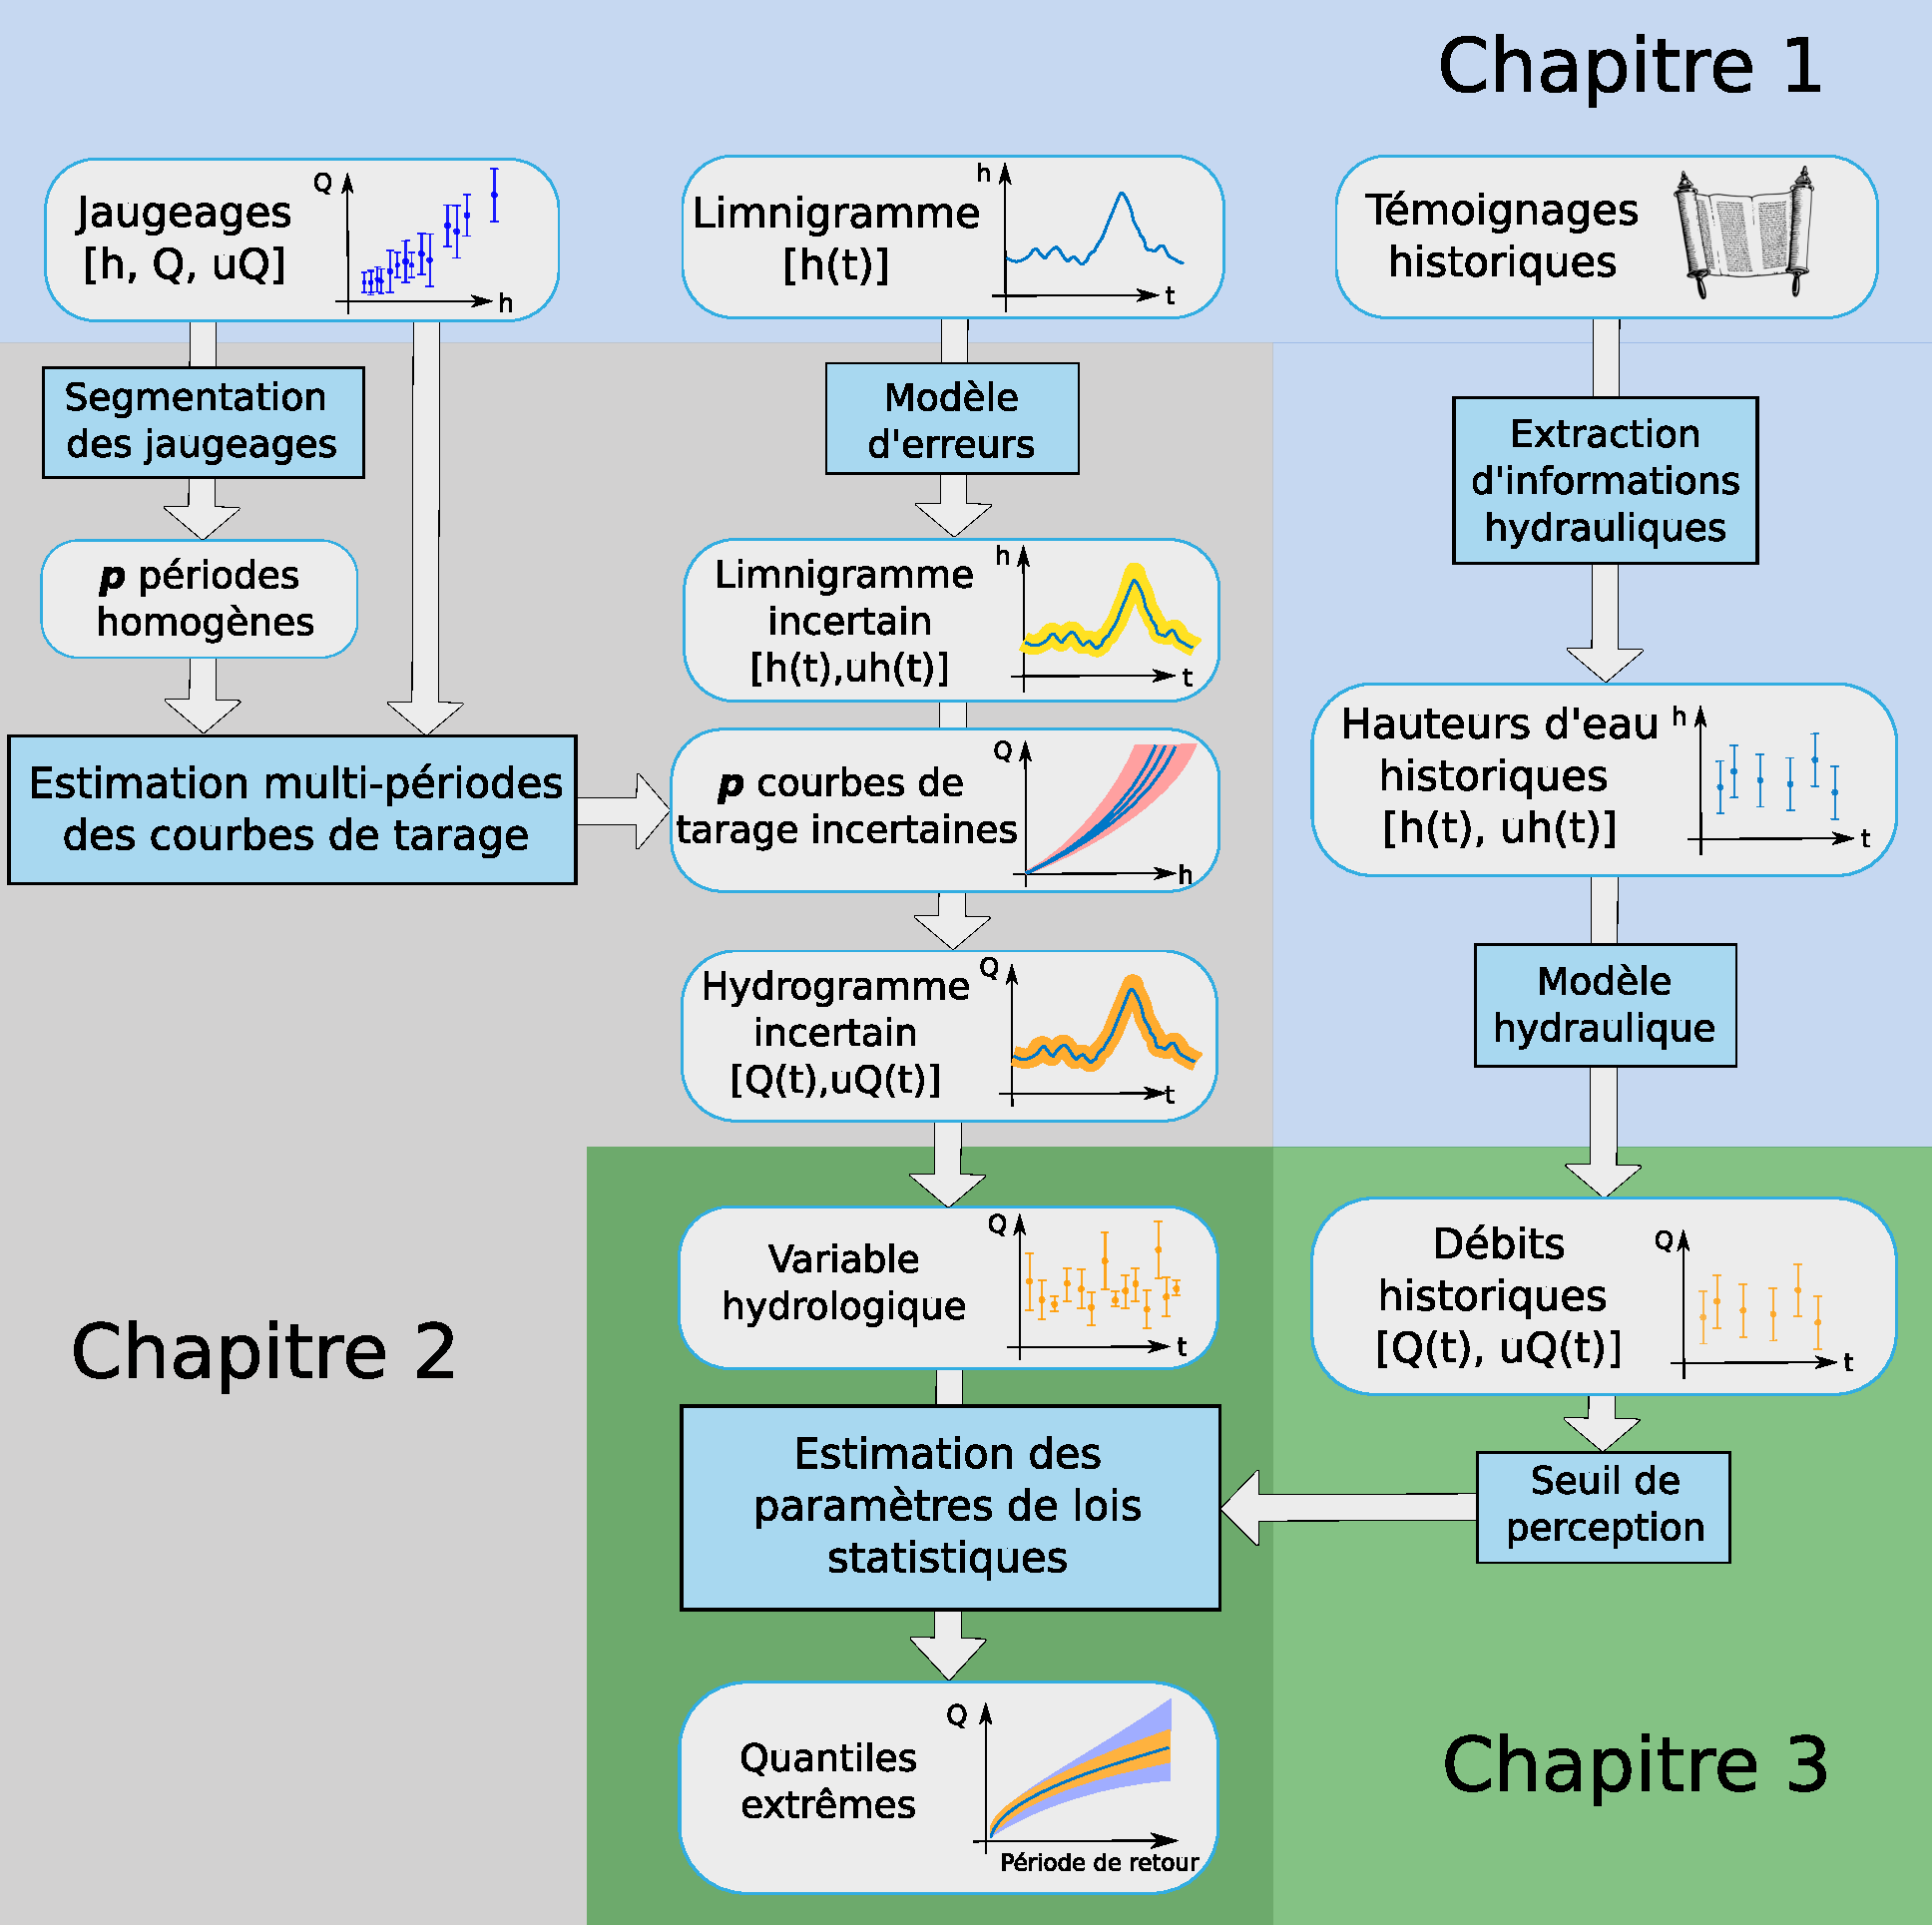
\includegraphics[width=.8\linewidth]{Figures/SchemaThese.pdf}	
	\caption{Schéma d'organisation de la thèse}
	\label{fig:SchemaThese}
\end{figure}

\FloatBarrier

\newpage

\printbibliography
\end{document}
